\subsection{The First Stars, Galaxies, \& Black Holes} \label{Sec: First Stars}
Immediately following the formation of the \gls{cmb}, a new cosmic epoch begins: The Dark Ages \citep{stark_galaxies_2016}. The Dark Ages are named so because it marks the period when no star formation took place. In this era, neutral, unionised hydrogen permeates the universe along with trace amounts of other metals (elements other than hydrogen and helium such as lithium and beryllium; \citealp{bromm_formation_2002, bromm_first_2004, gardner_james_2006}). Regions of space that were initially over-dense were the first to collapse under gravity and formed the very first objects in the universe \citep{barkana_beginning_2001}. This marked the end of The Dark Ages, approximately 200 million years after the Big Bang ($z\approx30$; \citealp{, gardner_james_2006}). 

These first stars, named population III (zero metallicity) stars, were the first objects to form in the universe and consisted entirely of hydrogen and helium gas. These stars had masses between 30 --- 300 $M_{\odot}$ and are thought to have produced the first core-collapse supernova and black holes, although this is still under debate \citep{magorrian_demography_1998, furlanetto_cosmology_2006, bromm_first_2011}. The immense pressure under the supernova produced heavier elements, eventually forming the population II and I stars (metal-poor and metal-rich, respectively) we see in the local universe today. The quantity and compactness of the available gas likely mean all black holes became either \gls{agn} or quasars \citep{loeb_reionization_2001}. Refer to \cref{Sec: Active Galactic Nuclei} for an introduction and review of \gls{agn}. UV emission and radiation from supernovas and quasars alike begin to ionise the universe. This marks the beginning of the \gls{eor}, likely between $z\approx15-30$ or 250-million years after The Big Bang and lasts until $z\approx6$ when the universe becomes highly ionised and the \gls{eor} ends \citep{loeb_reionization_2001, sokasian_cosmic_2004, fan_observational_2006}. 

% \begin{figure}[b!]
%     \setlength{\abovecaptionskip}{60pt} % Extra white space for video player
%     \embedvideo*{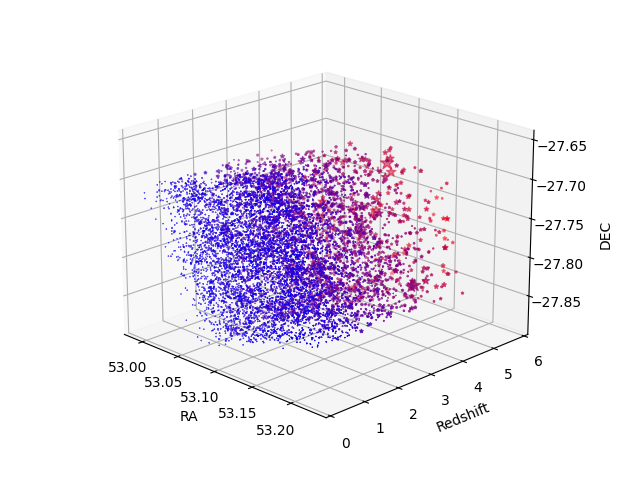
\includegraphics[width=\textwidth]{Figures/CDFS}}{Figures/CDFS.mp4}
%     \caption{Animated 3D-view of ZFOURGE CDFS field galaxies coloured by redshift.}
%     \setlength{\abovecaptionskip}{10pt} % Reset to default
%     \label{Fig: Animation}
% \end{figure}

\begin{figure}[b!]
    \centering
    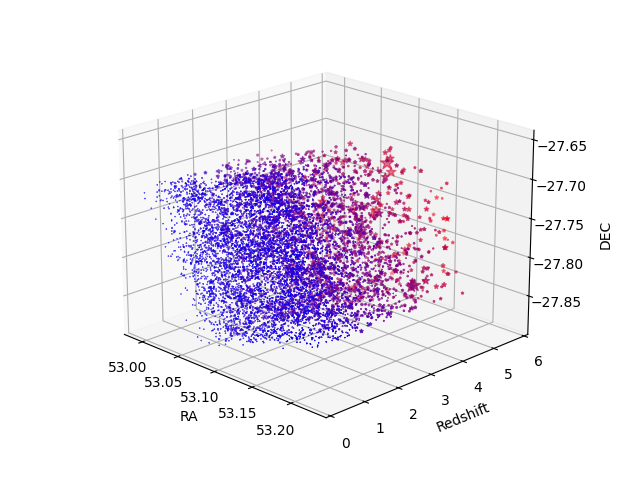
\includegraphics[width=\linewidth]{Figures/CDFS.png}
    \caption{The distribution of galaxies in the ZFOURGE CDFS field by \cite{lyon_decomposing_2024}. Sources are coloured by redshift and sized according to their total infrared luminosity. \href{https://www.youtube.com/watch?v=kTXSLjLGoNM}{Click here for animation.}}
    \label{Fig: Animation}
\end{figure}

The galaxies we observe in our local universe today are massive structures that have evolved from smaller ``building blocks" over time through mergers \citep{magorrian_demography_1998, ziparo_primordial_2024}. This has been the dominant perspective for the past 30 years. However, following the launch of the \gls{jwst} in December 2022, an alternative viewpoint has emerged: the existence of extraordinarily massive galaxies that formed so early in the universe's history challenges the ``building blocks" theory. \cite{labbe_population_2023} identifies six galaxies with stellar masses reaching up to $10^{11} M_{\odot}$ (more massive than the entire \textit{Milky Way}) within the redshift range of $7.4 \leq z \leq 9.1$. The discovery of such massive galaxies at these high redshifts is unprecedented and poses a significant challenge to \gls{lcdm} cosmology \citep{behroozi_most_2018, labbe_population_2023, greene_uncover_2024, bezanson_jwst_2024}. The available baryon budget is surpassed before $z=10$ \citep{menci_high-redshift_2022, boylan-kolchin_stress_2023}. This suggests that our current understanding and theoretical frameworks regarding mass accumulation and the evolution of the early universe may be flawed. It is also possible that the methods used may overestimate stellar mass, which should instead be attributed to \gls{agn} \citep{labbe_population_2023}, or that dark matter halos collapse much sooner than expected \citep{steinhardt_impossibly_2016}, but this necessitates new physics. Therefore, studies focusing on how less massive and fainter galaxies evolved at high redshift are crucial for comprehending the formation of the galaxies we observe today \citep{adams_discovery_2023, matthee_little_2024}.

The \gls{zfourge} survey \citep{straatman_fourstar_2016} is a significant study that aimed to investigate galaxies at higher redshifts, fainter luminosities, and lower masses than prior studies (\citealp{mcgreer_discovery_2006, dai_mid-infrared_2009, casey_redshift_2012, weiss_alma_2013} to name a few). ZFOURGE is designed to explore the evolution of galaxies, supermassive black holes, and \gls{agn} from high redshifts towards the end of the \gls{eor} ($z \approx 6$) to the present day ($z=0$). At a redshift of $z=6$, the universe is just 900 million years old \citep{astropy_collaboration_astropy_2022}. ZFOURGE allows researchers to track the evolution of galaxies over 93\% of the universe's history, particularly during critical cosmic epochs such as $1 < z < 3$, where luminosity density peaks before declining \citep{assef_mid-ir-_2011, gruppioni_modelling_2011, wylezalek_galaxy_2014, madau_cosmic_2014}. 

Figure \ref{Fig: Animation} showcases a 3D animation that illustrates the distribution of galaxies based on data from one field of the ZFOURGE survey (CDFS). Within the range of $1<z<6$, the co-moving distance to each galaxy varies between $3,000 \mathrm{Mpc}$ and $8,500 \mathrm{Mpc}$. Despite traversing thousands of Mpc, which should be significantly larger than necessary to observe \gls{lss}, discerning any extended formation remains challenging for several reasons. Although ZFOURGE investigates very deep redshifts, it operates as a pencil beam survey. The total surveying area of ZFOURGE is merely $0.1111$ deg$^2$ compared to the entire night sky, which spans 41,253 deg$^2$. In contrast, wide field surveys such as DESI \citep{desi_collaboration_desi_2016, desi_collaboration_desi_2024}, 2dF \citep{sadler_radio_2002, beutler_6df_2011}, and others \citep{mcgreer_discovery_2006, stevans_bridging_2018} can readily identify coherent structures. Despite this, the depth of observation achieved by the ZFOURGE survey and its ability to detect fainter celestial objects presents a substantial advantage in efforts towards constraining galaxy evolution. Because telescope time is finite, wide surveys and pencil-beam surveys balance area vs depth. Wide field surveys observe many objects over a large area but must spend less time per pointing, resulting in brighter flux limits. Pencil-beam surveys spend much longer observing small regions, enabling them to reach fainter flux limits.

The research currently being performed by \gls{jwst} will constrain the universe's evolution and inform the direction future research should follow. Indeed, the future directions are already taking shape \citep{labbe_population_2023}. The literature reveals a tension regarding the evolutionary path of galaxies and black holes from high redshift to the present day \citep{ziparo_primordial_2024}. The \gls{jwst} reveals massive galaxies that seemingly defy our existing frameworks and understanding. The new challenge is identifying galaxies with lower mass and luminosity at similarly high redshifts to analyse their evolution and, consequently, the build-up of mass in the earlier universe to constrain their evolution. This leads to the main focus of \cite{lyon_decomposing_2024}: investigating the link between \gls{sf} and the growth of BHs to better understand and constrain the universe's evolution over cosmic time.